% ACL/ARR master for the analysis/resource paper.
% Build (on a machine with TeX Live/MiKTeX):
%     pdflatex main && bibtex main && pdflatex main && pdflatex main
% or: latexmk -pdf main
%
% Table numbering here: T1 method comparison (S2), T2 per-class stage
% metrics (S4.5), T3 oracle ladder (S5), T4 failure fingerprints (S6.2).
% The Markdown master (../manuscript.md) uses the same numbering.

\documentclass[11pt]{article}
\usepackage[review]{acl}

\usepackage{times}
\usepackage{latexsym}
\usepackage[T1]{fontenc}
\usepackage[utf8]{inputenc}
\usepackage{microtype}
\usepackage{inconsolata}
\usepackage{graphicx}
\usepackage{booktabs}
\usepackage{longtable}
\usepackage{amsmath}
\usepackage{amssymb}
\usepackage{array}
\usepackage{multirow}

\graphicspath{{../figures/}{figures/}}

\title{Where Do Long-Term Memory Agents Lose Evidence?\\[2pt]
\large An audited attribution protocol, a corrected oracle ladder, and
architecture-conditional failure localisation}

\author{Anonymous ACL submission}

\begin{document}
\maketitle

\begin{abstract}
When a long-term memory agent answers incorrectly, accuracy benchmarks cannot
say where the failure happened. We present an attribution protocol that traces
each gold-evidence item through the system's lifecycle---formation, storage,
evolution, retrieval, context assembly, and answer reasoning (evolution is
exercised only on a controlled probe)---and localises the \emph{first
observable evidence-loss boundary} (F1--F6), with an explicit
evidence-insufficiency label (E0) for questions the gold evidence cannot
support. Because an attribution claim is only as good as its instruments, we
audit ours against 200 human-labelled questions: the failure labels are 90\%
human-confirmed, but the LLM judge systematically accepts abstention-style
answers (30.3\% of sampled stored-correct rows are human-wrong), and the
automatic evidence gate is near-independent of human sufficiency judgements
(Cohen's $\kappa$ 0.03--0.07) until rebuilt as a per-fact annotation task
($\kappa$ 0.835). We also show that the human \emph{stage} annotation task is
reliable ($\kappa$ 0.897) while the automatic first-loss label is not
(human-vs-auto $\kappa$ 0.59--0.71). Applying the corrected instruments, we
find that (i) the size of the memory-induced loss is benchmark-dependent: the
corrected real $\to$ oracle-memory $\to$ oracle-context ladder is
0.306 $\to$ 0.682 $\to$ 0.761 on LoCoMo (all rungs significant) but
0.479 $\to$ 0.676 $\to$ 0.799 on LongMemEval (last rung not significant); and
(ii) on LoCoMo $n{=}100$, three memory systems with statistically
indistinguishable accuracy (0.407/0.423/0.429; paired McNemar
$p = 0.736/0.728/0.864$) fail at significantly different lifecycle stages
(Stuart--Maxwell, Holm-adjusted $p \leq 2.8\times10^{-4}$ on all three pairs).
Two pre-registered architecture ablations move each system's dominant failure
stage in the predicted direction---but below the pre-registered magnitude
bar, so we report the localisation as \emph{architecture-conditional},
retract the stronger universal-fingerprint framing, and show that
stage-targeted repair does not beat a no-op placebo. We release the protocol,
the audit methodology, and all analysis artifacts as a resource for studying
memory-agent failure honestly.
\end{abstract}

\section{Introduction}

Long-term memory is becoming a standard component of LLM agents: conversation
history is written to a store, retrieved at answer time, and packed into the
model's context. Benchmarks such as LoCoMo and LongMemEval
\citep{maharana-etal-2024-locomo,wu2025longmemeval} measure how well such
systems answer questions over long histories, but their reported scores are
final-answer accuracy. When two systems score the same, accuracy alone cannot
distinguish \emph{where} each one fails---a system that never wrote the fact
looks identical to one that wrote it and never retrieved it. Repair effort,
and scientific understanding, require localising the failure.

This paper asks a measurement question: \textbf{can the earliest point at
which the evidence for an answer becomes unobservable be located reliably,
and does that location characterise how a memory system fails?} Our answer is
a qualified yes---with the qualifications being, we argue, the more useful
contribution.

Attribution itself is not a blank slate. HaluMem \citep{chen2025halumem}
introduced operation-level hallucination grading; MemOps
\citep{hao2026memops} benchmarks lifecycle operations on synthetic gold
traces; and MemTrace \citep{deng2026memtrace} formalises the earliest
\emph{decisive faulty operation} on an instrumented execution graph, with 160
human-annotated real failure cases. We therefore make \textbf{no priority
claim on lifecycle attribution}; \S\ref{sec:related} details the differences.
What the prior lines do not provide is a \emph{human-calibrated instrument}:
none reports pre-registered agreement between its judge and human labels, none
separates genuinely insufficient evidence from pipeline loss with controlled
oracle conditions, and none tests architecture-conditionality with a
pre-registered ablation gate. Those gaps are where this paper's claims live.

We make four contributions:

\begin{itemize}
\item \textbf{C1 --- An evidence-centric attribution protocol (\S\ref{sec:protocol}).}
A frozen pipeline that follows each benchmark question's gold-evidence items
through the artifacts a memory system exposes---formation, storage, evolution,
retrieval, context assembly, answer reasoning---and labels every wrong answer
with the \textbf{first observable evidence-loss boundary}: F1 formation,
F2 storage, F3 evolution, F4 retrieval, F5 context, F6 reasoning-candidate,
E0 evidence-insufficient, or EVAL (instrument uncertainty). The label is an
observability boundary, not a causal root cause; the protocol is explicit
about what it does not establish. It requires no source instrumentation, so it
applies to black-box systems; the trade-off is stage granularity rather than
operation- or code-level attribution.

\item \textbf{C2 --- A human audit of the instruments (\S\ref{sec:audit}).}
Two annotators labelled a stratified 200-question sample. The failure labels
are mostly sound (90\% confirmed), but the audit surfaces three instrument
defects that any LLM-judged memory study must handle: judge abstention false
positives (30.3\% of sampled stored-correct rows; a guarded correction rule is
13/13 precise where a naive rule is 52\%), an evidence-sufficiency gate that
is near-independent of humans ($\kappa$ 0.03--0.07) until rebuilt as per-fact
binary annotation (fact $\kappa$ 0.835, row $\kappa$ 0.889, after two failed
rounds), and a reliable human stage-annotation instrument ($\kappa$ 0.897)
against which the \emph{automatic} first-loss label is unreliable
($\kappa$ 0.59--0.71). We are not aware of a prior memory-failure study that
calibrates its judge and sufficiency gate against human labels under
pre-registered agreement bars and reports which conclusions the calibration
changes.

\item \textbf{C3 --- A corrected oracle ladder (\S\ref{sec:ladder}).}
Comparing real memory against oracle-memory and oracle-context controls
quantifies how much of the loss memory causes---but only after abstention
correction. No operation-level or execution-graph diagnostic from
\S\ref{sec:related} includes such controls. The corrected ladder is steep and
fully significant on LoCoMo (0.306 $\to$ 0.682 $\to$ 0.761) and shallower with
a non-significant final rung on LongMemEval (0.479 $\to$ 0.676 $\to$ 0.799):
the answer is benchmark-dependent, and corrections move individual rung
conclusions in both directions.

\item \textbf{C4 --- Architecture-conditional stage localisation
(\S\ref{sec:localisation}).} On LoCoMo $n{=}100$, three memory systems with
statistically indistinguishable accuracy fail at significantly different
lifecycle stages: a fact-extraction system loses evidence at formation, a
session-summary system at context assembly, a raw-turn RAG system at
retrieval. Cross-system differences in where failures occur have been
reported descriptively before (MemTrace, Fig.~4b); our addition is a
pre-registered within-system ablation with significance testing. Two ablations
that remove a system's own bottleneck move its dominant failure stage in the
pre-registered direction (A1: F1 share 0.13 $\to$ 0.00, within-system
Stuart--Maxwell $p = 0.0031$, accuracy unchanged; A3: F4 share 0.37 $\to$
0.23, accuracy $+17.6$ points)---but both miss the pre-registered
$\geq$20-point magnitude bar. The localisation is therefore real but
conditional on architecture, not a universal invariant of memory agents.
\end{itemize}

We state three negative results up front, because they delimit what the
positive claims mean. \textbf{(N1)} The stronger claim we initially
pursued---a stable, \emph{universal} failure fingerprint of memory agents---is
\textbf{retracted}: a pre-registered decision gate designed to test exactly
that claim returned a partial verdict, and the phenomenon is
architecture-conditional. \textbf{(N2)} Stage localisation is \textbf{not
shown to be actionable}: a pre-registered intervention that repairs the
measured retrieval stage moved retrieval recall 0.043 $\to$ 0.321 but produced
only +7 net answer flips (McNemar $p = 0.143$, bootstrap CI
$[-0.029, +0.441]$), inside the noise floor set by a no-op placebo (9/35
flips). \textbf{(N3)} The automatic first-loss label produced by the pipeline
is \textbf{not reliable as a per-row instrument} (human-vs-auto $\kappa$
0.59--0.71): it is dependable on formation/retrieval/none (per-class F1
0.81--1.00) but never emits E0 or rerank, so those two losses cannot be read
per row; stage-distribution claims are made on failure labels that the audit
found 90\% sound, at distribution level, and survive label noise drawn from
the measured confusion (\S\ref{sec:localisation}).

The paper is organised as a measurement study. \S\ref{sec:related} reviews
related work and states the positioning; \S\ref{sec:protocol} defines the
protocol; \S\ref{sec:audit} audits the instruments and states the reporting
rules we adopt; \S\ref{sec:ladder} and \S\ref{sec:localisation} present the
two substantive results; \S\ref{sec:repro} gives reproducibility detail; an
unnumbered limitations section follows, and Appendix~\ref{app:map} maps every
claim to the artifact that supports it.

\section{Related work}
\label{sec:related}

\subsection{Memory benchmarks}

LoCoMo \citep{maharana-etal-2024-locomo} established the now-standard
setting: long multi-session histories, questions posed afterwards,
final-answer scoring. LongMemEval \citep{wu2025longmemeval} organises
evaluation around five abilities---extraction, multi-session reasoning,
temporal reasoning, knowledge update, and abstention---and conceptualises a
memory system as a three-stage process of indexing, retrieval, and reading.
MemBench \citep{tan-etal-2025-membench} separates factual from reflective
memory and adds efficiency and capacity dimensions; MemoryAgentBench
\citep{hu2025memoryagentbench} frames evaluation as incremental multi-turn
interaction across four competencies; RealMem \citep{bian2026realmem}
interleaves queries inside the interaction; LoCoMo-Plus
\citep{li2026locomoplus} probes implicit constraints and cognitive memory.

These benchmarks differ in coverage, not in what a score means: a system is
judged on the correctness of its final answers. LongMemEval's stage
vocabulary notwithstanding, none reports, for a wrong answer, where along the
system's own pipeline the required evidence first stopped being available.
That is the question this paper measures. An attribution protocol is
orthogonal to benchmark choice---it consumes whatever gold evidence a
benchmark provides---which is why we run it on two benchmarks rather than
proposing a third.

\subsection{Operation-level and lifecycle diagnostics}

Three recent lines have moved inside the pipeline, and we state the
relationship to each explicitly because one of them defines our problem.

\textbf{HaluMem} \citep{chen2025halumem} introduced operation-level
hallucination grading: gold memory points and update pairs are annotated, and
a memory system is scored separately on extraction, updating, and question
answering over synthetic user histories. It shows that extraction and update
errors arise and propagate to QA---a pipeline-level pattern our stage labels
also expose---but its gold states are benchmark-generated, its scoring is a
single automatic judge without human calibration (human annotation validates
dataset quality, not the scoring instrument), and retrieval enters only
through recall. It measures whether prescribed memory operations are performed
correctly; it does not localise where evidence became unavailable for an
observed real failure.

\textbf{MemOps} \citep{hao2026memops} benchmarks whether systems can
\emph{detect, execute, and respect} lifecycle operations---remember, forget,
update, reflect, and their compositions---embedded in synthetic conversations
with gold operation traces and six probe families (detection, target binding,
state transition, disambiguation, application, state trajectory). Its question
is ``can the system detect and carry out the right operation, and respect the
resulting memory state?'', ours is ``for a question the system already
answered wrongly, which stage of its own pipeline first stopped exposing the
evidence?'' The authors list stronger human validation and judge-calibration
studies as future work; we perform that calibration.

\textbf{MemTrace} \citep{deng2026memtrace} is the closest work and the reason
this paper makes no priority claim on lifecycle attribution. It formalises the
problem as locating the \emph{earliest decisive faulty operation} in an
execution graph obtained by instrumenting the system's source code; it builds
MemTraceBench---160 human-annotated failure cases from LoCoMo, LongMemEval,
and RealMem over four systems (Long-Context, RAG, Mem0, EverMemOS)---and
reports operation-identification accuracy from 14\% (GPT-4.1 mini) to 58\%
(GPT-5.4 with source-evidence and pipeline-prior signals), plus a
prompt-optimisation application. Its taxonomy distinguishes annotation errors
(gold evidence insufficient for the reference answer---our E0) and LLM-judge
errors, which we also treat as first-class labels. We differ along four axes:

\begin{enumerate}
\item \textbf{Object of tracing.} MemTrace follows operations and variables in
an instrumented graph; we follow the gold evidence items for a question
through whatever artifacts the system exposes (store, retrieved items,
assembled context). Ours needs no source instrumentation and therefore applies
to black-box systems, but it cannot name the faulty line of code, and it
inherits the benchmark's gold-evidence completeness.
\item \textbf{Instrument calibration.} MemTrace records but excludes
annotation and judge errors during benchmark construction (67 and 3 of 230
annotated cases) without quantifying the judge's error rates. Our audit
measures them---30.3\% abstention false positives, gate--human $\kappa$
0.03--0.07, a rebuilt per-fact gate at $\kappa$ 0.835---and shows which paired
conclusions the correction changes.
\item \textbf{Controlled conditions.} MemTrace compares systems as they are; we
add an oracle ladder (real memory / oracle memory / oracle context) that
attributes loss to memory versus context versus answer generation. None of the
lifecycle-diagnostic lines above includes such controls.
\item \textbf{Pre-registered ablation.} MemTrace reports that error
distributions differ across systems (its Fig.~4b) as a descriptive finding. We
test the same kind of observation with a pre-registered decision gate and
within-system ablations, and we report the gate as partial rather than
renegotiating the bar after seeing the result.
\end{enumerate}

Table~\ref{tab:methods} summarises the comparison. Entries are read from the
papers unless marked $\dagger$, which are measured in this work; there is no
head-to-head run, because the four artifacts do not share a question set with
per-system traces and gold evidence (Limitations).

\begin{table*}[t]
\centering
\small
\setlength{\tabcolsep}{3.5pt}
\begin{tabular}{@{}p{2.1cm}p{3.2cm}p{2.8cm}p{2.8cm}p{4.2cm}@{}}
\toprule
dimension & MemTrace & HaluMem & MemOps & this work \\
\midrule
observability requirement & instrumented source code & memory-system APIs &
memory-system APIs & black-box artifacts only \\
granularity & operation / variable & operation (extraction, updating, QA) &
operation (5 types) $+$ probes & lifecycle stage on gold evidence \\
data & real benchmarks $\times$ 4 systems; 160 annotated failures & synthetic;
$\sim$15k memory points & synthetic; 4{,}012 instances & real benchmarks
$\times$ 3 systems; 200-row audit $+$ 40-row stage pilot \\
judge calibration & judge errors recorded (3/230), rate not measured & none
reported & none (listed as future work) & answer $\kappa$ 0.92; abstention
rule 13/13$^\dagger$; gate $\kappa$ 0.835$^\dagger$; stage $\kappa$
0.897$^\dagger$; per-class stage audit$^\dagger$ \\
attribution vs.\ humans & OIA 14--58\% & n/a (no failure attribution) & n/a &
per-row stage $\kappa$ 0.59--0.71; per-class F1 0.81--1.00$^\dagger$ \\
controls & none & none & none & RM/OM/OC oracle ladder$^\dagger$ \\
applicability & systems that can be instrumented & systems with the three APIs
& systems with the APIs & any system exposing its store, retrievals, and
context \\
\bottomrule
\end{tabular}
\caption{Attribution methods compared. Entries are from the cited papers
unless marked $\dagger$, which are measured in this work. No head-to-head run
exists (see Limitations).}
\label{tab:methods}
\end{table*}

\subsection{Memory systems}

We cite the major architectural families as context, not as evaluated
systems: extraction-and-update stores \citep{chhikara2025mem0}, context-window
operating systems \citep{packer2023memgpt}, agentic note-organisation
\citep{xu2025amem}, graph-augmented retrieval \citep{gutierrez2024hipporag},
earlier self-controlled and session-summary memory
\citep{wang2024scm,pan2025secom}, and unified memory operating layers
\citep{li2025memos}. The three systems we evaluate (\S\ref{sec:localisation})
are controlled implementations that instantiate the extraction, compression,
and raw-turn-retrieval families. We do not claim they are the strongest
members of their families; they are chosen so that each carries a known,
removable bottleneck, which is what the ablation requires.

\subsection{Reliability of automatic evaluation}

LLM-as-judge studies document systematic biases---position and verbosity bias
\citep{zheng2023judging,wang2024notfairevaluators}, prompt-sensitivity in
reference-based scoring \citep{liu2023geval}, and self-preference
\citep{panickssery2024selfpreference}---and later work systematises bias
families \citep{ye2025justice,chen2024humansjudge,shi2025judgingjudges}.
Inter-annotator agreement has a long methodological literature
\citep{artstein2008kappa}.

Our audit targets a specific failure mode that generic bias studies do not
isolate: in a memory pipeline, the judge \textbf{rewards abstention}. Of
sampled rows the judge stored as correct, 30.3\% are human-adjudicated wrong,
and 13 of 20 are abstention-style answers accepted as correct. Because
abstention is a first-class capability in LongMemEval
\citep{wu2025longmemeval}, a naive ``abstention is wrong'' correction is only
52\% precise; guarding on the reference answer makes it 13/13 precise on the
sampled subset. The point is not that judges are biased---that is
established---but that in this task the correction \emph{moves paired
significance conclusions} (\S\ref{sec:ladder}), which a bias inventory does
not show.

\subsection{Failure attribution in agent systems}

Attribution methods for agent trajectories localise faulty steps within a
single task run---via sampling and process signals, LLM inspection of traces,
or structured graphs \citep{zhang2025whoandwhen,agentracer2025,bonagiri2026causalflow};
see also the MAS failure taxonomy of \citet{cemri2025whymasfail}. Memory
failures violate their core assumption: the faulty step may lie many sessions
before the observed failure, and the trace is not a short ordered log.
MemTrace extends graph-based attribution to memory with instrumentation; we
take the protocol route---observable artifacts, gold evidence, no
instrumentation---and pay for it in granularity. The two routes are
complementary, and the audit of \S\ref{sec:audit} applies to either.

\section{The attribution protocol}
\label{sec:protocol}

The protocol observes only what a memory system exposes---what it writes, what
it retrieves, and what it assembles into the answer context---so it applies to
black-box deployments; it never reads a system's source code or requires
instrumentation. Its ground-truth signal is each benchmark's own gold evidence.

\subsection{Conditions}

The protocol runs each benchmark question under up to three conditions:

\begin{itemize}
\item \textbf{Real Memory (RM).} The benchmark conversation is ingested by the
real memory system; the answer is produced from retrieved context.
\item \textbf{Oracle Memory (OM).} The gold evidence is written directly into a
fresh store as raw turns and retrieved through the real
retrieval/rerank/context path. Formation and storage are controlled (direct
write) and reported as unmeasured; retrieval, rerank, and context are measured.
\item \textbf{Oracle Context (OC).} The gold evidence is placed directly in the
answer context. All stages before context are unmeasured.
\end{itemize}

The RM $\to$ OM $\to$ OC ladder isolates how much accuracy is recovered when
upstream stages are progressively perfectioned (\S\ref{sec:ladder}).

\begin{figure}[t]
\centering
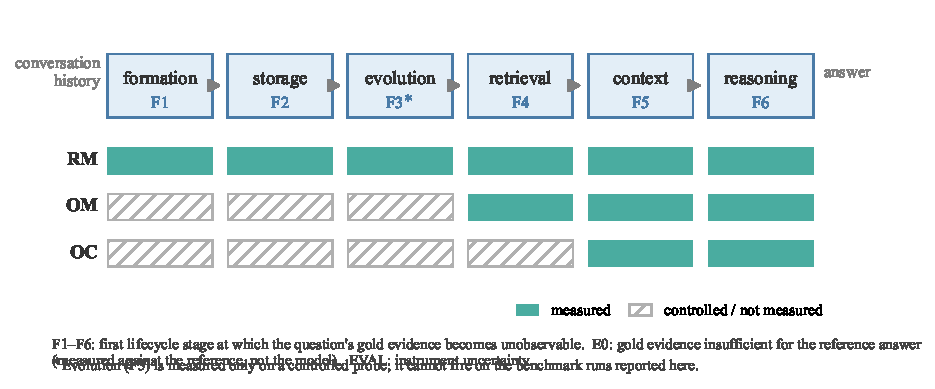
\includegraphics[width=\linewidth]{fig1_lifecycle.pdf}
\caption{Lifecycle stages and the three conditions. Each question's gold
evidence is followed through six lifecycle stages; F1--F6 mark the first stage
at which it becomes unobservable. The lower matrix shows which stages each
condition measures (solid) or controls (hatched). E0 labels evidence
insufficiency measured against the reference answer; EVAL marks instrument
uncertainty. $^{\ast}$Evolution (F3) is measured only on a controlled probe.}
\label{fig:lifecycle}
\end{figure}

\subsection{Lifecycle stages and evidence matching}

For each question, the benchmark provides gold evidence items with provenance
(session/turn identifiers). The tracer measures, at each stage, the recall of
the gold evidence in that stage's artifacts:
formation $\to$ storage $\to$ evolution $\to$ retrieval $\to$ rerank $\to$
context. A gold item is matched by exact normalized text, or by token-overlap
similarity $\geq 0.55$, among provenance-compatible artifacts. Provenance is a
constraint, not proof: an artifact whose turn conflicts with the gold
provenance cannot satisfy the item; a match in an artifact without provenance
is reported separately rather than hidden. Evolution (F3) is measured only on
datasets whose adapter exposes an atomic-fact store with supersession
(currently a controlled evolution probe); on the benchmark runs reported here
the stage is skipped and F3 cannot fire.

\subsection{First observable evidence-loss boundary}

\emph{Terminology.} We report the \textbf{first observable evidence-loss
boundary}---the earliest stage at which the evidence required for the
reference answer stops being observable along the traced pipeline. We
deliberately do \emph{not} call this a causal root cause: the boundary says
where evidence became unobservable, not which internal mechanism
counterfactually caused the wrong answer. (Where ``first-loss'' appears in
code and artifacts it is shorthand for this boundary.)

\subsection{Answer evaluation and failure labels}

Model answers are judged semantically against the benchmark reference, with
deterministic floors around the judge: pre-judge lexical support, post-judge
repair restricted to question-related candidates (never refusals), and a
false-overturn \emph{ordering-refutation} layer for two-option ordering
questions whose evidence resolves the dates. Failure attribution then assigns,
in order:

\begin{enumerate}
\item semantically correct $\to$ no failure;
\item no semantic verdict $\to$ \texttt{EVAL\_SEMANTIC\_UNCERTAIN};
\item evidence gate insufficient $\to$ \texttt{E0\_EVIDENCE\_INSUFFICIENT};
\item gate not sufficient / low confidence $\to$ \texttt{EVAL};
\item Oracle-Context mode $\to$ \texttt{RC\_REASONING\_CONTROL\_FAILURE};
\item no gold evidence ids $\to$ \texttt{E0};
\item first measured stage missing gold $\to$ F1/F2/F4/F5;
\item all evidence present in context $\to$ \texttt{F6\_REASONING\_CANDIDATE}.
\end{enumerate}

The evidence-sufficiency gate (E0) is judged \textbf{against the benchmark
reference answer, never the model prediction}, so it is non-circular. F6 is a
\emph{candidate}: it means the evidence reached the context and the answer was
still wrong, which is consistent with a reasoning failure but also with
evaluation error---the audit of \S\ref{sec:audit} quantifies both.

\subsection{Label versions and reporting discipline}

The audit (\S\ref{sec:audit}) shows the raw automatic labels carry measurable
instrument error. We therefore track three label versions and state, for every
number, which version it uses:

\begin{itemize}
\item \textbf{auto} --- the stored automatic judge/gate labels;
\item \textbf{abstention-corrected} --- auto labels with the human-validated
abstention rule applied (\S\ref{sec:audit}); used for all accuracy-level
claims;
\item \textbf{human-gated} --- abstention-corrected labels with the E0 gate
replaced by the two-annotator consensus gate on annotated questions
(\S\ref{sec:audit}); used to re-attribute E0 on covered questions.
\end{itemize}

Accuracy is reported as \emph{semantic accuracy on judged rows} (rows with a
judge verdict), never as the fraction of all rows marked correct, which
understates accuracy. E0 is reported only as a relative pattern across
conditions, never as an error-rate level, except where the human gate covers
the question.

\subsection{What the protocol does not establish}

Three boundaries are stated in the protocol itself: (i) labels are
observability boundaries, not causal mechanisms; (ii) F6 is a candidate class,
not a measured reasoning failure; (iii) per-row first-loss reads are not
validated as a per-row instrument (N3)---stage claims are made at the
distribution level, on labels whose failure direction the audit found 90\%
sound.

\section{Auditing the instruments}
\label{sec:audit}

An attribution paper makes two kinds of claim: that an answer was wrong, and
that a particular lifecycle boundary was where the evidence first became
unobservable. Both rest on instruments---a semantic judge and an
evidence-sufficiency gate---and if those instruments are not audited, the
attribution map is a map of instrument error. This section reports the audit;
it absorbs and supersedes our earlier standalone instrument note.

\subsection{Audit design}

Two annotators independently labelled a stratified 200-question sample (100
LoCoMo $+$ 100 LongMemEval) drawn from the canonical $n{=}200$ runs, blind to
the stored verdicts; every disagreement was adjudicated. Fields: answer
correctness and evidence sufficiency. A separate 40-question package (two
further annotators) measured the reliability of \emph{stage} annotation
against the automatic first-loss label (\S\ref{sec:audit:stage}).

\subsection{Answer correctness is measurable; failure labels are mostly sound}

Inter-annotator agreement on answer correctness is high ($\kappa = 0.92$,
$n = 177$ co-decided; the 7 disagreements were paraphrase/equivalence cases,
adjudicated correct). Against the adjudicated labels, the automatic judge
reaches precision 0.697 / recall 0.885 / F1 0.780 overall ($\kappa = 0.591$),
with a large per-benchmark gap: LoCoMo F1 0.605 ($\kappa$ 0.369) vs
LongMemEval F1 0.880 ($\kappa$ 0.747).

The base rate that every stage claim rests on survives review: of 60
stored-incorrect rows with a human verdict, \textbf{54 (90.0\%) are confirmed
wrong}. The direction of the failure labels does not rest on the gate.

\subsection{The judge rewards abstention; a guarded rule corrects it}

Of 66 sampled rows the judge stored as semantically correct, \textbf{20
(30.3\%) are human-adjudicated wrong}, and 13 of the 20 are abstention-style
answers (``Not mentioned'', ``Cannot be determined'') that the judge accepted.
Left uncorrected, semantic accuracy is inflated wherever a model declines to
answer---and the oracle conditions are inflated most, because they abstain
least often for the wrong reason.

The correction is label-only and human-validated. A naive rule (``a
stored-correct abstention is wrong'') is only \textbf{52\% precise} on the 25
sampled abstentions, because 12 are LongMemEval \texttt{\_abs} questions whose
reference answer is itself an abstention. Guarding on the reference (flip only
when the reference is a concrete proposition) identifies \textbf{all 13
human-wrong abstentions and preserves all 12 human-correct ones} (precision
and recall 1.00 on the abstention subset). On the full 77-row stored-correct
sample the rule flips 13 of 31 human-wrong rows (recall 0.42); the remaining
18 are non-abstention judge errors the rule does not address---we do not claim
otherwise.

\subsection{The evidence gate needed three rounds to become an instrument}

The round-1 sufficiency field was degenerate ($\kappa = 0.0$: one annotator
never said ``no''; all 20 disagreements adjudicated against the lenient side).
A round-2 derivability checklist still failed ($\kappa = 0.181$, $n = 177$):
one annotator's ``missing fact'' notes were a mechanical template lifting
tokens from the reference answer---75/81 quoted tokens occur in the reference,
0/81 in the evidence, including function words (``she'', ``because''). Round 3
changed the task shape: each reference answer is decomposed once into atomic
propositions (276 facts over 200 questions), and annotators mark one binary
fact-presence judgement per row; the row gate is a transparent aggregation.
This instrument cleared its pre-registered bar ($\kappa \geq 0.6$ on both
levels):

\begin{table}[t]
\centering
\small
\begin{tabular}{@{}lrr@{}}
\toprule
measure & value & bar \\
\midrule
fact-level $\kappa$ ($n = 234$ co-decided) & \textbf{0.835} (agreement 0.970) & 0.6 \\
row-level $\kappa$, uncertain $\to$ insufficient ($n = 200$) & \textbf{0.889} & 0.6 \\
row-level $\kappa$, excluding uncertain ($n = 172$) & 0.830 & 0.6 \\
\bottomrule
\end{tabular}
\caption{Round-3 per-fact gate: both pre-registered bars cleared.}
\label{tab:gate}
\end{table}

Against the 200 adjudicated labels (178 consensus rows), the consensus gate
reaches precision 0.837 / recall 1.000 / F1 0.911, versus the stored gate's
0.244 / 0.528 / 0.333 on the same rows. Because the fact decomposition was
authored with access to the adjudicated labels, we treat the inter-annotator
$\kappa$ as the independent validation and the adjudication comparison as
corroboration.

The stored automatic gate is near-independent of humans ($\kappa$ 0.03--0.07).
In the direction that matters for E0, it \textbf{falsely marks 65 sufficient
rows insufficient} (28 LoCoMo, 37 LongMemEval---the latter dominated by
\texttt{\_abs} questions, whose reference is itself an abstention) and
\textbf{misses 17 truly-insufficient rows} (all LoCoMo): the error is
dominated by over-flagging. Consequently, E0 counts from the automatic gate
are biased upward and are used only for relative comparison across conditions
of the same question (one shared gate per question); on annotated questions we
re-attribute with the consensus gate, which removes 5--10 E0 rows per mode
(human-gated vs corrected labels: LoCoMo real 56 $\to$ 51, OM 40 $\to$ 30, OC
30 $\to$ 25; LongMemEval real 13 $\to$ 5, OM 13 $\to$ 8, OC 15 $\to$ 8),
converting them to F1/F4/F6/RC. Questions outside the annotated sample keep
the stored gate and the caveat.

\subsection{The human stage instrument is reliable; the automatic first-loss label is not}
\label{sec:audit:stage}

A separate two-annotator package asked humans to assign the first
evidence-loss stage on 40 LoCoMo questions from the $n{=}100$ fingerprint run,
with full retrieval/context previews and an explicit ``preview absence = stage
missing'' rule. After a failed v1 ($\kappa = 0.685$ on valid rows; 13/40 rows
used an unmeasured label), the v2 instrument passed its pre-registered bar:
agreement 0.925, \textbf{multiclass $\kappa = 0.897$} (bar 0.70), no uncertain
rows.

Against the human labels, the automatic first-loss label reaches only
$\kappa = 0.705$ (annotator a) and $\kappa = 0.590$ (annotator b). The
disagreements concentrate on E0 (humans call 4 rows E0 where the automatic
trace assigns formation/retrieval) and on rerank (humans see 3 rerank losses
the automatic label calls retrieval). \textbf{The human stage instrument is
reliable; the automatic first-loss label is not a per-row instrument.} All
stage-distribution claims in \S\ref{sec:localisation} are therefore made at
the distribution level on failure labels (90\% human-confirmed,
\S\ref{sec:audit}), not on per-row first-loss reads.

\textbf{Where exactly the automatic label errs.} Per-class quantities on the
consensus rows ($n = 37$ where both annotators agree; consensus
$\kappa = 0.680$, agreement 0.784---a filtered subset, not directly
comparable to the per-annotator $\kappa$ above):

\begin{table}[t]
\centering
\small
\begin{tabular}{@{}lrrrrr@{}}
\toprule
class & support & predicted & precision & recall & F1 \\
\midrule
formation & 8 & 8 & 0.875 & 0.875 & 0.875 \\
retrieval & 15 & 22 & 0.682 & 1.000 & 0.811 \\
none & 7 & 7 & 1.000 & 1.000 & 1.000 \\
e0 & 4 & 0 & --- & 0.000 & --- \\
rerank & 3 & 0 & --- & 0.000 & --- \\
\bottomrule
\end{tabular}
\caption{Per-class performance of the automatic stage label against the
human consensus (40-row pilot; 37 consensus rows). The label never emits E0 or
rerank.}
\label{tab:perclass}
\end{table}

The instrument is dependable on the classes it emits---formation F1 0.88, none
1.00, retrieval 0.81 (recall 1.00, precision 0.68 because it absorbs the
misplaced E0/rerank rows)---and its errors are structural rather than noisy:
it \textbf{never emits E0 or rerank}. Human E0 losses are absorbed into
formation (1 row) and retrieval (3 rows); human rerank losses into retrieval
(3 rows). Read per row, the label is therefore a usable
formation/retrieval/none classifier and structurally unable to separate E0
from pipeline loss or rerank from retrieval; read as a distribution, it
carries the signal \S\ref{sec:localisation} uses.
\S\ref{sec:localisation} tests the conclusion against noise drawn from exactly
this confusion matrix.

\subsection{Reporting rules we adopt and recommend}

Three rules, which we follow throughout and suggest for any LLM-judged
memory-failure study:

\begin{enumerate}
\item \textbf{Floor first.} Ship deterministic, auditable rules for label
dimensions that admit one (temporal equivalence, ordering refutation,
abstention detection) before trusting a judge.
\item \textbf{Report the $\kappa$.} Every judge-derived dimension is reported
with its human agreement; a dimension below the pre-registered bar is marked
non-citable (for us: automatic E0 levels and per-row first-loss labels).
\item \textbf{Report both label versions.} Auto and corrected numbers appear
together; the corrected number is the headline and the delta is the
measurement error.
\end{enumerate}

\section{How much of the loss is memory? The corrected oracle ladder}
\label{sec:ladder}

The RM $\to$ OM $\to$ OC ladder (\S\ref{sec:protocol}) quantifies how much
accuracy is recovered when formation/storage (OM) and then everything upstream
of the answer (OC) are perfectioned. Table~\ref{tab:ladder} reports semantic
accuracy on judged rows, $n = 200$ per benchmark, on both label versions
(\S\ref{sec:protocol}).

\begin{table}[t]
\centering
\small
\setlength{\tabcolsep}{3pt}
\begin{tabular}{@{}llrrrrrr@{}}
\toprule
benchmark & labels & RM & OM & OC & RM$\to$OM & RM$\to$OC & OM$\to$OC \\
\midrule
LoCoMo & auto & 0.405 & 0.832 & 0.852 & $<$1e-3 & $<$1e-3 & 0.541 \\
LoCoMo & corrected & \textbf{0.306} & \textbf{0.682} & \textbf{0.761} &
4.3e-12 & 2.3e-17 & \textbf{0.0146} \\
LongMemEval & auto & 0.521 & 0.691 & 0.821 & 0.004 & $<$1e-3 & 0.041 \\
LongMemEval & corrected & \textbf{0.479} & \textbf{0.676} & \textbf{0.799} &
1.6e-4 & 4.2e-7 & \textbf{0.078 (n.s.)} \\
\bottomrule
\end{tabular}
\caption{Oracle ladder, auto vs abstention-corrected labels ($n = 200$).
$p$ values: exact McNemar on discordant pairs. On corrected labels, paired
bootstrap CIs exclude 0 for every contrast except LongMemEval OM$\to$OC, whose
CI reaches 0. Judged rows: LoCoMo 173/173/176; LongMemEval 163/139/134.}
\label{tab:ladder}
\end{table}

\begin{figure}[t]
\centering
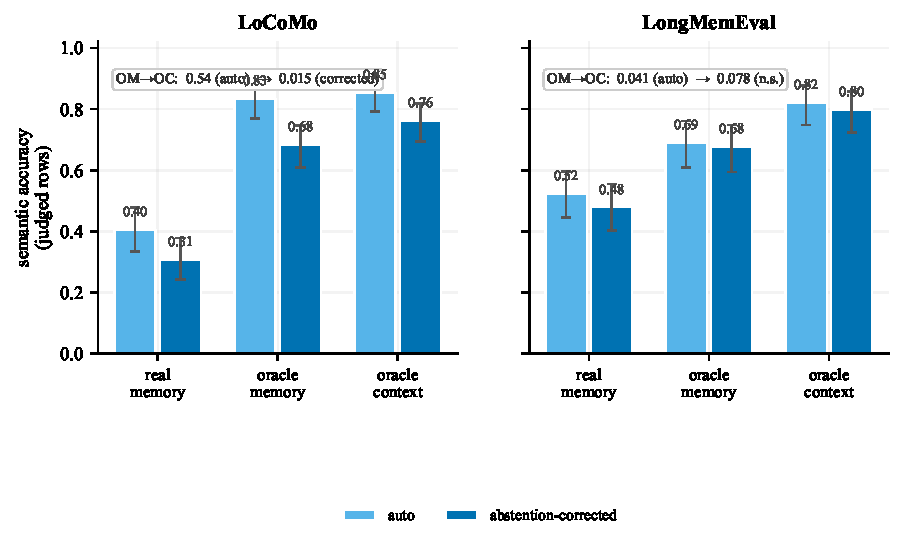
\includegraphics[width=\linewidth]{fig2_ladder.pdf}
\caption{Oracle ladder, auto vs abstention-corrected labels ($n = 200$). Bars
are semantic accuracy on judged rows with Wilson 95\% CIs. The abstention
correction moves the final rung in opposite directions on the two benchmarks:
LoCoMo OM$\to$OC becomes significant (0.54 $\to$ 0.015), LongMemEval stops
being significant (0.041 $\to$ 0.078).}
\label{fig:ladder}
\end{figure}

Three observations:

\begin{itemize}
\item \textbf{The correction moves individual conclusions in both directions.}
On LoCoMo, counting abstentions as wrong makes the final OM$\to$OC rung
\emph{significant} (0.541 $\to$ 0.0146); on LongMemEval it makes the same rung
\emph{non-significant} (0.041 $\to$ 0.078). Oracle modes absorb the most new
E0 rows (LoCoMo OM $+25$, OC $+16$), because they abstain least often for the
wrong reason---the auto ladder flattered them.
\item \textbf{The size of the memory-induced loss is benchmark-dependent.} On
LoCoMo, real memory loses two-thirds of the judged accuracy that oracle memory
recovers, and perfecting the context still adds a significant rung---after
gold is in memory, the remaining loss is retrieval/context. On LongMemEval,
the real$\to$OM recovery is smaller and the last rung does not separate. A
single ``memory costs $X$ points'' number would be an artifact of benchmark
choice.
\item \textbf{The ladder is a control, not a ceiling.} OM/OC absorb E0 (43\%
of LoCoMo questions are gate-insufficient under the automatic gate), so ladder
rungs are reported alongside the gate caveat of \S\ref{sec:audit} and are
never read as error rates.
\end{itemize}

\section{Failure-stage localisation is architecture-conditional}
\label{sec:localisation}

\subsection{Three systems with known bottlenecks}

We run three memory systems through the same questions, judge, gate,
deterministic floors, and 6000-character context budget:

\begin{itemize}
\item \textbf{semantic} --- an LLM extracts atomic facts per turn
(provenance-carrying), with governance superseding stale facts; retrieval over
the fact store. \emph{Designed bottleneck:} formation (extraction can drop or
distort facts).
\item \textbf{summary} --- one LLM summary per session, no per-fact provenance.
\emph{Designed bottleneck:} context (compression loses detail).
\item \textbf{verbatim} --- raw conversation turns, cosine retrieval (windowed
RAG). \emph{Designed bottleneck:} retrieval (raw-turn similarity ranks
poorly).
\end{itemize}

We name the bottlenecks explicitly because they matter to the interpretation:
the systems were \emph{authored} with these bottlenecks, so a stage difference
is evidence about architecture, not about memory agents in general
(\S\ref{sec:localisation:gate}).

\subsection{Same accuracy, different failure stage (LoCoMo $n = 100$)}

Table~\ref{tab:fingerprint} reports the one-batch run (100 questions $\times$
3 systems, shared per-question gate, errors 0; auto labels; accuracy =
semantic accuracy on judged rows).

\begin{table*}[t]
\centering
\small
\begin{tabular}{@{}lcp{3.7cm}p{7.0cm}@{}}
\toprule
system & acc (judged) & formation / retrieval / context recall & failure distribution \\
\midrule
semantic & 0.407 (91) & 0.473 / 0.424 / 0.303 &
none 42, E0 21, \textbf{F1 18}, F4 14, F5 1, EVAL 4 \\
summary & 0.423 (97) & 0.990 / 0.990 / 0.258 &
none 42, E0 23, \textbf{F5 21}, F4 10, F6 1, EVAL 3 \\
verbatim & 0.429 (98) & 0.990 / \textbf{0.197} / 0.162 &
none 43, E0 19, \textbf{F4 35}, F6 1, EVAL 2 \\
\bottomrule
\end{tabular}
\caption{Cross-system fingerprint, LoCoMo $n = 100$, auto labels.}
\label{tab:fingerprint}
\end{table*}

\begin{figure}[t]
\centering
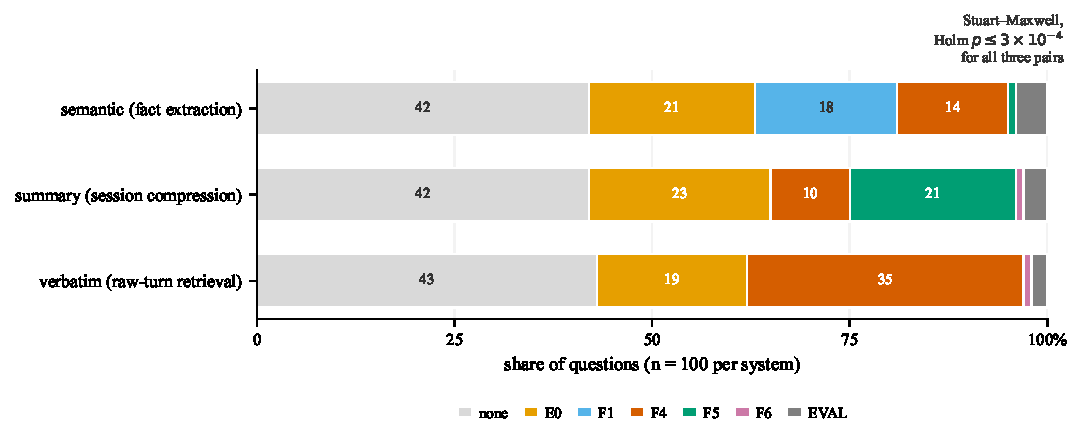
\includegraphics[width=\linewidth]{fig3_fingerprint.pdf}
\caption{Failure-stage distributions, LoCoMo $n = 100$. Segment widths are
shares of 100 questions per system; numerals are counts. End accuracy is
statistically indistinguishable across systems while the stage distributions
differ for all three pairs (statistics in the text and Table~\ref{tab:fingerprint}).}
\label{fig:fingerprint}
\end{figure}

End accuracy is statistically indistinguishable across all pairs (exact
McNemar $p = 0.736 / 0.728 / 0.864$; paired bootstrap CIs all include 0). The
failure-stage distributions are significantly different for \textbf{all three
pairs}: Stuart--Maxwell $p = 7.4\times10^{-5}$ (semantic vs summary),
$2.7\times10^{-4}$ (semantic vs verbatim), $5.0\times10^{-5}$ (summary vs
verbatim); Holm-adjusted $\leq 2.8\times10^{-4}$ throughout; the paired
max-abs permutation test agrees ($p = 0.0045 / 0.0007 / <0.0001$). Per-label
paired bootstrap CIs isolate the pattern: semantic's F1 share is $+0.18$ over
both others (CI $[0.11, 0.26]$), summary's F5 share $+0.21$ over verbatim (CI
$[0.13, 0.29]$; $-0.20$ vs semantic, CI $[-0.29, -0.12]$), verbatim's F4
share $+0.21$ over semantic (CI $[0.12, 0.30]$) and $+0.25$ over summary (CI
$[0.15, 0.35]$).

\subsection{The distribution result does not depend on E0 or on the automatic gate}

Two sensitivity results, both pre-registered as Stage A of the decision plan:

\begin{itemize}
\item \textbf{E0-excluded.} Dropping the 42 questions whose shared gate is not
sufficient (58 used), all three pairs remain significant: $p = 2.0\times10^{-5}
/ 7.5\times10^{-5} / 2.7\times10^{-5}$, Holm-adjusted $\leq 7.6\times10^{-5}$.
The headline does not depend on the (upward-biased, \S\ref{sec:audit}) E0
class.
\item \textbf{Human instrument.} The human stage-annotation instrument is
reliable ($\kappa = 0.897$, \S\ref{sec:audit:stage}); the automatic label's
per-row unreliability ($\kappa$ 0.59--0.71) is why claims are made on
distributions of 90\%-confirmed failure labels, and the E0-excluded variant
removes the class where human and automatic labels disagree most.
\item \textbf{Label-noise sensitivity.} Monte Carlo over the stored
$n{=}100$ failure labels (300 draws per cell): each row's label is redrawn
with probability $q$ from (A) the empirical auto$\to$human confusion measured
on the 40-row pilot, or (B) a uniform swap over the observed classes
(adversarial). Under (A), all three pairs keep Stuart--Maxwell
$p < 0.05$ in \textbf{100\% of draws at every} $q \in
\{0.1, 0.2, 0.3, 0.5\}$---the conclusion survives the misclassification the
instrument actually exhibits. Under (B), survival at $q = 0.5$ falls to 0.31
(semantic vs verbatim), 0.73 (semantic vs summary), 0.88 (summary vs
verbatim); at $q \leq 0.2$ it stays $\geq 0.88$ throughout. The headline
therefore does not require the automatic label to be correct row by row, but
it is not immune to arbitrary relabeling.
\item \textbf{Pilot consistency.} On the 40 annotated rows, human and
automatic labels agree on each system's dominant stage (semantic: formation;
verbatim: retrieval), though the counts differ where the automatic trace folds
E0 and rerank losses into formation/retrieval (\S\ref{sec:audit:stage}).
\end{itemize}

\subsection{Ablations and the pre-registered gate: partial, not passed}
\label{sec:localisation:gate}

Stage B of the frozen decision plan tests whether the fingerprint tracks
architecture: turn off a system's own bottleneck and check whether its
dominant failure stage moves. The pre-registered pass rule requires, for
\textbf{at least two of three} systems, (i) the dominant-stage share moves
\textbf{$\geq 20$ percentage points} and (ii) the within-system
Stuart--Maxwell $p < 0.05$ survives Holm. Two conditions were run (A2, the
summary-bottleneck condition, was deferred before any run because a smoke test
showed context assembly, not summary lossiness, binds). Each ablation is a
self-contained paired $n{=}100$ batch with its own shared gate; baseline
numbers therefore differ slightly across batches and are never compared
cross-batch.

\textbf{A1 --- remove the formation bottleneck} (semantic vs
\texttt{semantic\_rawwrite} write-through verbatim storage). The mechanism
responds exactly as pre-registered: formation recall 0.473 $\to$ 0.990, F1
13 $\to$ 0 rows, and retrieval failures double (F4 12 $\to$ 24) as the loss
relocates downstream. Per-label paired bootstrap: F1 $+0.13$ (CI
$[0.07, 0.20]$), F4 $-0.12$ (CI $[-0.22, -0.03]$). The within-system
Stuart--Maxwell is significant ($\chi^2 = 19.75$, df $= 6$,
\textbf{$p = 0.0031$}, Holm 0.0031; permutation $p = 0.0394$)---the first
ablation condition where the stage-distribution test itself clears $\alpha$.
Accuracy is unchanged (0.500 vs 0.430, McNemar $p = 0.392$, CI
$[-0.054, +0.185]$): the same system, the same accuracy, a different failure
location. \textbf{But the largest share move is 13 points---below the
20-point bar.}

\textbf{A3 --- remove the retrieval bottleneck} (verbatim vs hybrid ranking).
Retrieval recall 0.197 $\to$ 0.402; F4 share 0.37 $\to$ 0.23 (14 points);
accuracy improves 0.351 $\to$ 0.527 (McNemar $p = 0.014$). The within-system
Stuart--Maxwell is $p = 0.066$ (permutation $p = 0.0087$). \textbf{14 points,
below the bar; the distribution test does not clear Holm.}

\textbf{Verdict: partial.} 0 of 2 evaluated conditions pass both criteria, and
the decision gate returns \emph{partial}. Two protocol facts are recorded with
the verdict and must travel with it: (i) with A2 deferred, only two of three
systems were evaluable, so the ``$\geq$2 of 3'' rule \textbf{could not} return
a pass under the executed design; and (ii) the 20-point bar couples to base
rate---F1 was 13\% of rows in the A1 batch, so \emph{eliminating} formation
failure could move that share by at most 13 points. The direction criterion
was met in both conditions; the magnitude criterion was not. Per the frozen
decision plan, we therefore \textbf{narrow the claim}: the localisation
phenomenon is reported as architecture-conditional, and the
universal-fingerprint framing is retracted (N1). We do not restate the bar
after the fact.

\subsection{Cross-benchmark check: qualitative only}

On the only locally available full-haystack LongMemEval sample ($n = 10$,
${\sim}$50 sessions per record), the failure labels again differ across
systems (verbatim: 4 retrieval losses; summary: retrieval/context losses;
semantic: no retrieval losses). At $n = 10$ this is a sanity check, not
evidence; the limitations section lists the missing second-benchmark
replication.

\subsection{Stage localisation is not shown to be actionable (N2)}

The pre-registered intervention repaired the measured retrieval stage on the
35 F4 questions of the $n{=}100$ run (hybrid candidate widening). The
mechanism worked (retrieval recall 0.043 $\to$ 0.321), but the paired outcome
did not clear the decision rule ($\geq 6$ net flips \textbf{and} bootstrap CI
lower bound $> 0$): net \textbf{+7} flips, McNemar $p = 0.143$, bootstrap
diff $+0.206$, 95\% CI $[-0.029, +0.441]$. A no-op placebo that simply
re-asks the question flipped 9/35 (${\approx}26\%$) of the same subset---the
+7 net sits inside that retest noise. A stage-agnostic composite arm reaches
0.563 overall accuracy (vs 0.429 baseline) but is \emph{worse} on the 65 non-F4
questions (42 $\to$ 38 correct), so the repair is not stage-exclusive.
\textbf{Measurement validity and intervention validity must be kept apart}:
the measurement is valid---the F4 class is real and the repaired mechanism
moved recall as designed---while the intervention is not shown to be
effective; the null is evidence about actionability, not about the attribution
signal. Contribution: a measured stage is not, at this power, an actionable
repair target; Stage C of the decision plan is not started.

\section{Reproducibility}
\label{sec:repro}

\begin{itemize}
\item \textbf{Frozen configuration.} Commit \texttt{b8b1f6e}, branch
\texttt{fix/formation-diagnostics-evidence-based}; freeze document
\texttt{docs/PROTOCOL\_FREEZE.md}; every post-freeze change is logged in
\texttt{docs/PRE\_REGISTRATION\_CHANGELOG.md} before the affected run.
\item \textbf{Models.} DeepSeek-v4.1-flash for answer, judge (temperature 0),
and gate (temperature 0); embedding backend recorded per run in
\texttt{run\_metadata}.
\item \textbf{Statistics.} Exact McNemar \citep{mcnemar1947} on discordant
pairs; paired bootstrap (5{,}000--10{,}000 repeats, seed 42); Stuart--Maxwell
\citep{stuart1955,maxwell1970} with Holm correction \citep{holm1979} across the
three-pair family; max-abs paired permutation (10{,}000 repeats, seed 42).
Wilson CIs \citep{wilson1927} for accuracy; Cohen's $\kappa$
\citep{cohen1960} for agreement.
\item \textbf{Code and tests.} The protocol, tracer, evaluator, systems,
runners, and all analysis scripts are in the repository; 232 unit tests pass.
Every analysis number in this paper regenerates from stored rows by label-only
re-computation (no model calls) via the scripts named in Appendix~\ref{app:map}.
\item \textbf{Data.} LoCoMo (refined public split) and LongMemEval are public
benchmarks; the annotation packages (blinded worksheets, keys, adjudicated
labels) and all \texttt{results/analysis\_*.json} artifacts are released with
the repository. Raw per-row model outputs are reconstructable from the
recorded run metadata.
\item \textbf{Compute.} All runs are CPU-only apart from the answer/judge/gate
API; the largest batch ($n = 200 \times 3$ conditions) runs on a single
workstation.
\end{itemize}

\section*{Limitations}

\begin{itemize}
\item \textbf{Single-benchmark headline.} C4 rests on LoCoMo $n{=}100$; the
second real-haystack benchmark is an $n{=}10$ qualitative pilot
(\S\ref{sec:localisation}). External validity is open.
\item \textbf{Embedding backend.} Every reported run uses the deterministic
in-process \texttt{hash:384} embedding fallback; comparisons are valid only
within that backend. The retrieval bottleneck is not an embedding artifact: on
the 35 F4 questions, a real 1024-d embedding (bge-m3, served locally) raises
dense recall only 0.043 $\to$ 0.100 and hybrid recall 0.321 $\to$ 0.343, while
overall dense recall is not higher (0.106 under bge-m3 vs 0.205 stored hash).
\item \textbf{Single judge.} One model (DeepSeek-v4.1-flash, temperature 0)
produced every answer, judgement, and gate decision; no second-model protocol
was approved. Within-judge self-consistency is perfect ($\kappa = 1.0$); the
cross-family robustness of judge verdicts is unmeasured here, and earlier
exploratory cross-model reads (quarantined) are not cited.
\item \textbf{Instrument caveats travel with the numbers.} Fingerprint labels
come from the automatic gate (E0 biased upward; \S\ref{sec:audit}); failure
labels are 90\% human-confirmed; the abstention correction is a validated
rule, not per-row human labels on the full runs; the human consensus gate
covers 200 of the 400 $n{=}200$ questions.
\item \textbf{Stage B evaluated two of three conditions} (A2 deferred), and
the gate's pass rule was arithmetically unreachable under the executed design
(\S\ref{sec:localisation:gate}).
\item \textbf{No head-to-head comparison with the operation-diagnostic
benchmarks.} HaluMem, MemOps, and MemTraceBench each define their own systems
and gold annotations; our protocol is applied only to our own three systems,
so the comparison in \S\ref{sec:related} is architectural, not an empirical
ranking. A shared evaluation would need a common question set with gold
evidence and per-system traces, which none of the four artifacts provides
together.
\item \textbf{Evolution (F3)} is measured only on a controlled probe, not on
the benchmark runs; nothing here quantifies evolution-stage loss in the wild.
\end{itemize}

\section*{Ethical considerations}

The study uses two public benchmarks and internally produced annotations; no
new human-subject data was collected beyond task annotation carried out within
the project. Annotator disagreement data is reported in aggregate. Because the
paper's subject is the \emph{unreliability of automated instrumentation}, we
flag the residual risk that our corrected labels still carry the errors
quantified in \S\ref{sec:audit}, and we release the annotation packages so the
corrections can themselves be re-audited.

\bibliographystyle{acl_natbib}
\bibliography{references}

\appendix

\section{Claim $\to$ artifact map}
\label{app:map}

Every quantitative claim in this paper regenerates from the stored artifacts
below (all under \texttt{results/}, label-only recomputation unless noted).
Raw \texttt{comparison*.jsonl} rows are local by policy; the analysis
artifacts and the generating scripts are tracked.

\small
\begin{longtable}{@{}p{6.0cm}p{5.2cm}p{4.3cm}@{}}
\toprule
claim & artifact(s) & script \\
\midrule
\endhead
Protocol semantics, label versions, decision order &
\texttt{docs/PROTOCOL.md}, \texttt{docs/PROTOCOL\_FREEZE.md} &
\texttt{evaluation/attribution.py} \\
Answer $\kappa$ 0.92; gate $\kappa$ 0.0; judge P/R/F1; 54/60 failure labels
confirmed; 20/66 abstention FPs &
\texttt{analysis\_annotations\_adjudicated\_n200.json} &
\texttt{experiments/score\_annotations.py} \\
Stored gate near-independent (65 false-insufficient / 17 missed) &
\texttt{analysis\_gate\_confusion\_n200.json} &
\texttt{experiments/analyze\_gate\_confusion.py} \\
Round-2 gate failure ($\kappa$ 0.181; template pathology) &
\texttt{analysis\_annotations\_round2\_diagnostic.json} &
\texttt{experiments/diagnose\_gate\_annotations.py} \\
Round-3 fact gate ($\kappa$ 0.835 / 0.889; P/R/F1 0.837/1.000/0.911) &
\texttt{analysis\_annotations\_round3.json} &
\texttt{experiments/score\_fact\_annotations.py} \\
Abstention rule: naive 52\% vs guarded 13/13 \& 12/12 &
\texttt{analysis\_abstention\_rule\_validation.json} &
\texttt{experiments/validate\_abstention\_rule.py} \\
Corrected ladder (Table~\ref{tab:ladder}), both label versions &
\texttt{analysis\_ladder\_\{locomo,longmemeval\}\_n200\_\{auto,corrected\}.json} &
\texttt{experiments/analyze\_ladder.py} \\
Human-gated E0 re-attribution &
\texttt{analysis\_regate\_\{locomo,longmemeval\}\_n200.json} &
\texttt{experiments/regate\_with\_human\_gate.py} \\
Human stage annotation $\kappa$ 0.897; human-vs-auto $\kappa$ 0.705/0.590 &
\texttt{analysis\_round5\_pilot\_v2.json} &
\texttt{experiments/score\_stage\_annotations.py} \\
Per-class stage metrics; label-noise sensitivity &
\texttt{analysis\_stage\_label\_audit.json} &
\texttt{experiments/audit\_stage\_labels.py} \\
$n{=}100$ fingerprint (Table~\ref{tab:fingerprint}), paired tests &
\texttt{analysis\_ladder\_locomo\_n100\_fixedgate.json} &
\texttt{experiments/analyze\_ladder.py} \\
E0-excluded stage tests &
\texttt{analysis\_stage\_excluding\_e0\_locomo\_n100.json} &
\texttt{experiments/analyze\_stage\_excluding\_e0.py} \\
A1 ablation (formation recall 0.473 $\to$ 0.990; SM $p = 0.0031$) &
\texttt{analysis\_ablation\_a1\_n100.json} &
\texttt{analyze\_ladder} on \texttt{systems\_ablation\_n100\_a1/} \\
A3 ablation (recall 0.197 $\to$ 0.402; SM $p = 0.066$) &
\texttt{analysis\_ablation\_a3\_n100.json} &
\texttt{analyze\_ladder} on \texttt{systems\_ablation\_n100\_a3/} \\
Gate-B verdict and pre-registered criteria &
\texttt{decision\_gate\_b.json} & \texttt{experiments/emit\_decision\_gate.py} \\
Route decision, claim re-scope, retractions &
\texttt{route\_decision\_2026-10-27.json} & (decision record) \\
Intervention null (+7 net, $p = 0.143$, CI $[-0.029, +0.441]$; placebo 9/35) &
\texttt{retrieval\_intervention\_locomo\_n100/summary.json} &
\texttt{experiments/retrieval\_intervention.py} \\
bge-m3 embedding check &
\texttt{embedding\_backend\_check\_locomo\_n100.json\{,l\}} &
\texttt{experiments/check\_embedding\_retrieval.py} \\
LongMemEval full-haystack pilot ($n = 10$) &
\texttt{analysis\_ladder\_longmemeval\_sample10\_fixedgate.json} &
\texttt{experiments/analyze\_ladder.py} \\
Adversarial review motivating the decision plan &
\texttt{docs/reviews/2026-10-26-direction-kill-argument.md} & --- \\
Governing decision plan, gates A--D &
\texttt{docs/CCF\_B\_DECISION\_PLAN\_2026-10-26.md} & --- \\
\bottomrule
\end{longtable}
\normalsize

\section{Gate-B decision artifact (verbatim criteria)}
\label{app:gateb}

The pre-registered rule evaluated by \texttt{results/decision\_gate\_b.json}:

\begin{quote}
\textbf{Pass:} for at least two of the three systems, turning off its
bottleneck (1) changes that system's dominant-stage share by
$\geq 20$ percentage points, and (2) the within-system Stuart--Maxwell
$p < 0.05$ survives Holm across the three tests. \textbf{Fail:} all three
knobs leave the dominant-stage share within $\pm 10$ points and no
within-system test is significant. \textbf{Between:} reported as partial; the
claim is narrowed to the systems/conditions where the stage moved.
\end{quote}

Evaluated: A1 (13-point move, Holm $p = 0.0031$ $\to$ criterion 2 met,
criterion 1 not) and A3 (14-point move, Holm $p = 0.066$ $\to$ neither
criterion). A2 deferred before any run. Verdict: \textbf{partial}; claim
narrowed to architecture-conditional localisation; universal fingerprint
retracted; route switched to the analysis/resource paper (this manuscript).
Recorded in \texttt{results/route\_decision\_2026-10-27.json} and the
pre-registration changelog entry of 2026-10-27.

\end{document}
